% Résumé du principe de l'expérience

\subsection{Matériel}
% Liste du matériel
Le matériel suivant a été nécessaire a la réalisation des expériences:\\
\begin{itemize}
	\item Un générateur de fréquence
	\item Un oscilloscope
	\item Des câbles (dont 2 avec une mise à terre)
	\item 2 résistance (5 et 50 [$\Omega$])
    \item Un condensateur (1 [$\mu F$])
    \item Une bobine (3 [$m H$])
\end{itemize}

\subsection{Déroulement}
% Déroulement de l'expérience
Avant de débuter l'expérience, il est nécessaire d'assembler le matériel comme présenté dans la section schéma (\ref{sec:schema}), vérifier le fonctionnement correct de l'oscilloscope.\\

La tension $U$, $U_{in}$ et la fréquence $f$ sont données sur la page principale de l'oscilloscope. Afin de trouver notre écart $\Delta t$, utiliser les curseurs manuels est incontournable. Une fois la page de curseurs ouverte, il est nécessaire de placer l'un d'entre eux au sommet d'une courbe, puis de l'autre. De cette manière, la valeur de $\Delta t$ s'affichera.
\begin{figure}[H]
  \centering
    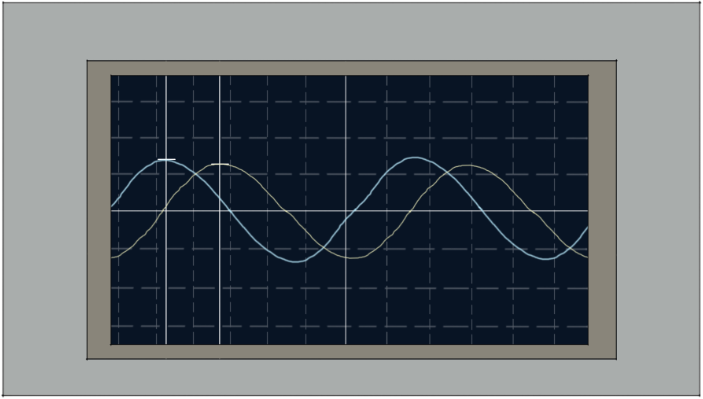
\includegraphics[width=0.6\textwidth]{phy_osci.PNG}
    \caption{Schéma de l'oscilloscope}
\end{figure}

\subsubsection*{Expérience 1 :}
\begin{itemize}
    \item Assembler le circuit en utilisant la résistance de 50 [$\Omega$].
    \item Commencer à 10 [$Hz$]
    \item Pour chaque mesure, prendre note de la fréquence [$Hz$], de la tension [$V$], de la tension induite [$V$], et de $\Delta t$ [$s$].
    \item "Doubler" la fréquence jusqu'à 10 [$kHz$] (10, 20, 50, 100, 200, ...).
    \item Faire de même avec la résistance de 5 [$\Omega$].
\end{itemize}

\subsubsection*{Expérience 2 :}

\begin{itemize}
    \item Assembler le circuit en utilisant la résistance de 50 [$\Omega$].
    \item Commencer à 5 [$Hz$]
    \item Pour chaque mesure, prendre note de la fréquence [$Hz$], de la tension [$V$], de la tension induite [$V$], et de $\Delta t$  [$s$].
    \item "Doubler" la fréquence jusqu'à 20 [$kHz$] (5, 10, 20, 50, 100, 200, ...).
\end{itemize}

\subsection{Schémas}
\label{sec:schema}
% Schéma avec légende
\subsubsection*{Expérience 1 :}

\begin{minipage}{.5\textwidth}
\begin{figure}[H]
  \centering
    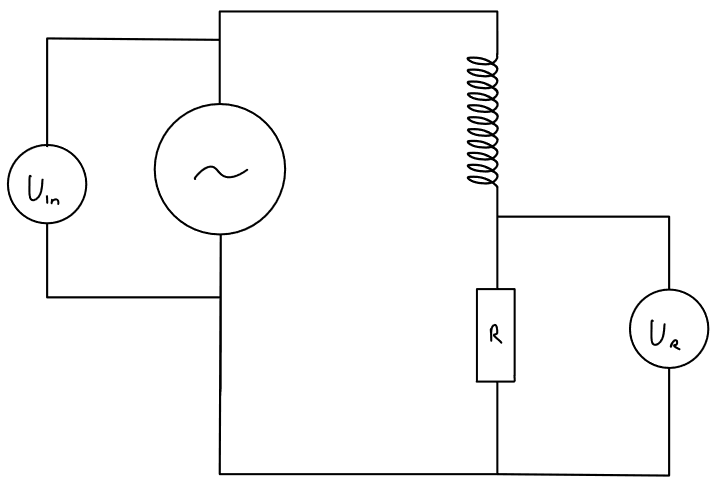
\includegraphics[width=0.8\textwidth]{phy_cir_RL.PNG}
    \caption{Schéma du circuit $RL$}
\end{figure}
\end{minipage}
\begin{minipage}{.5\textwidth}
\begin{figure}[H]
  \centering
    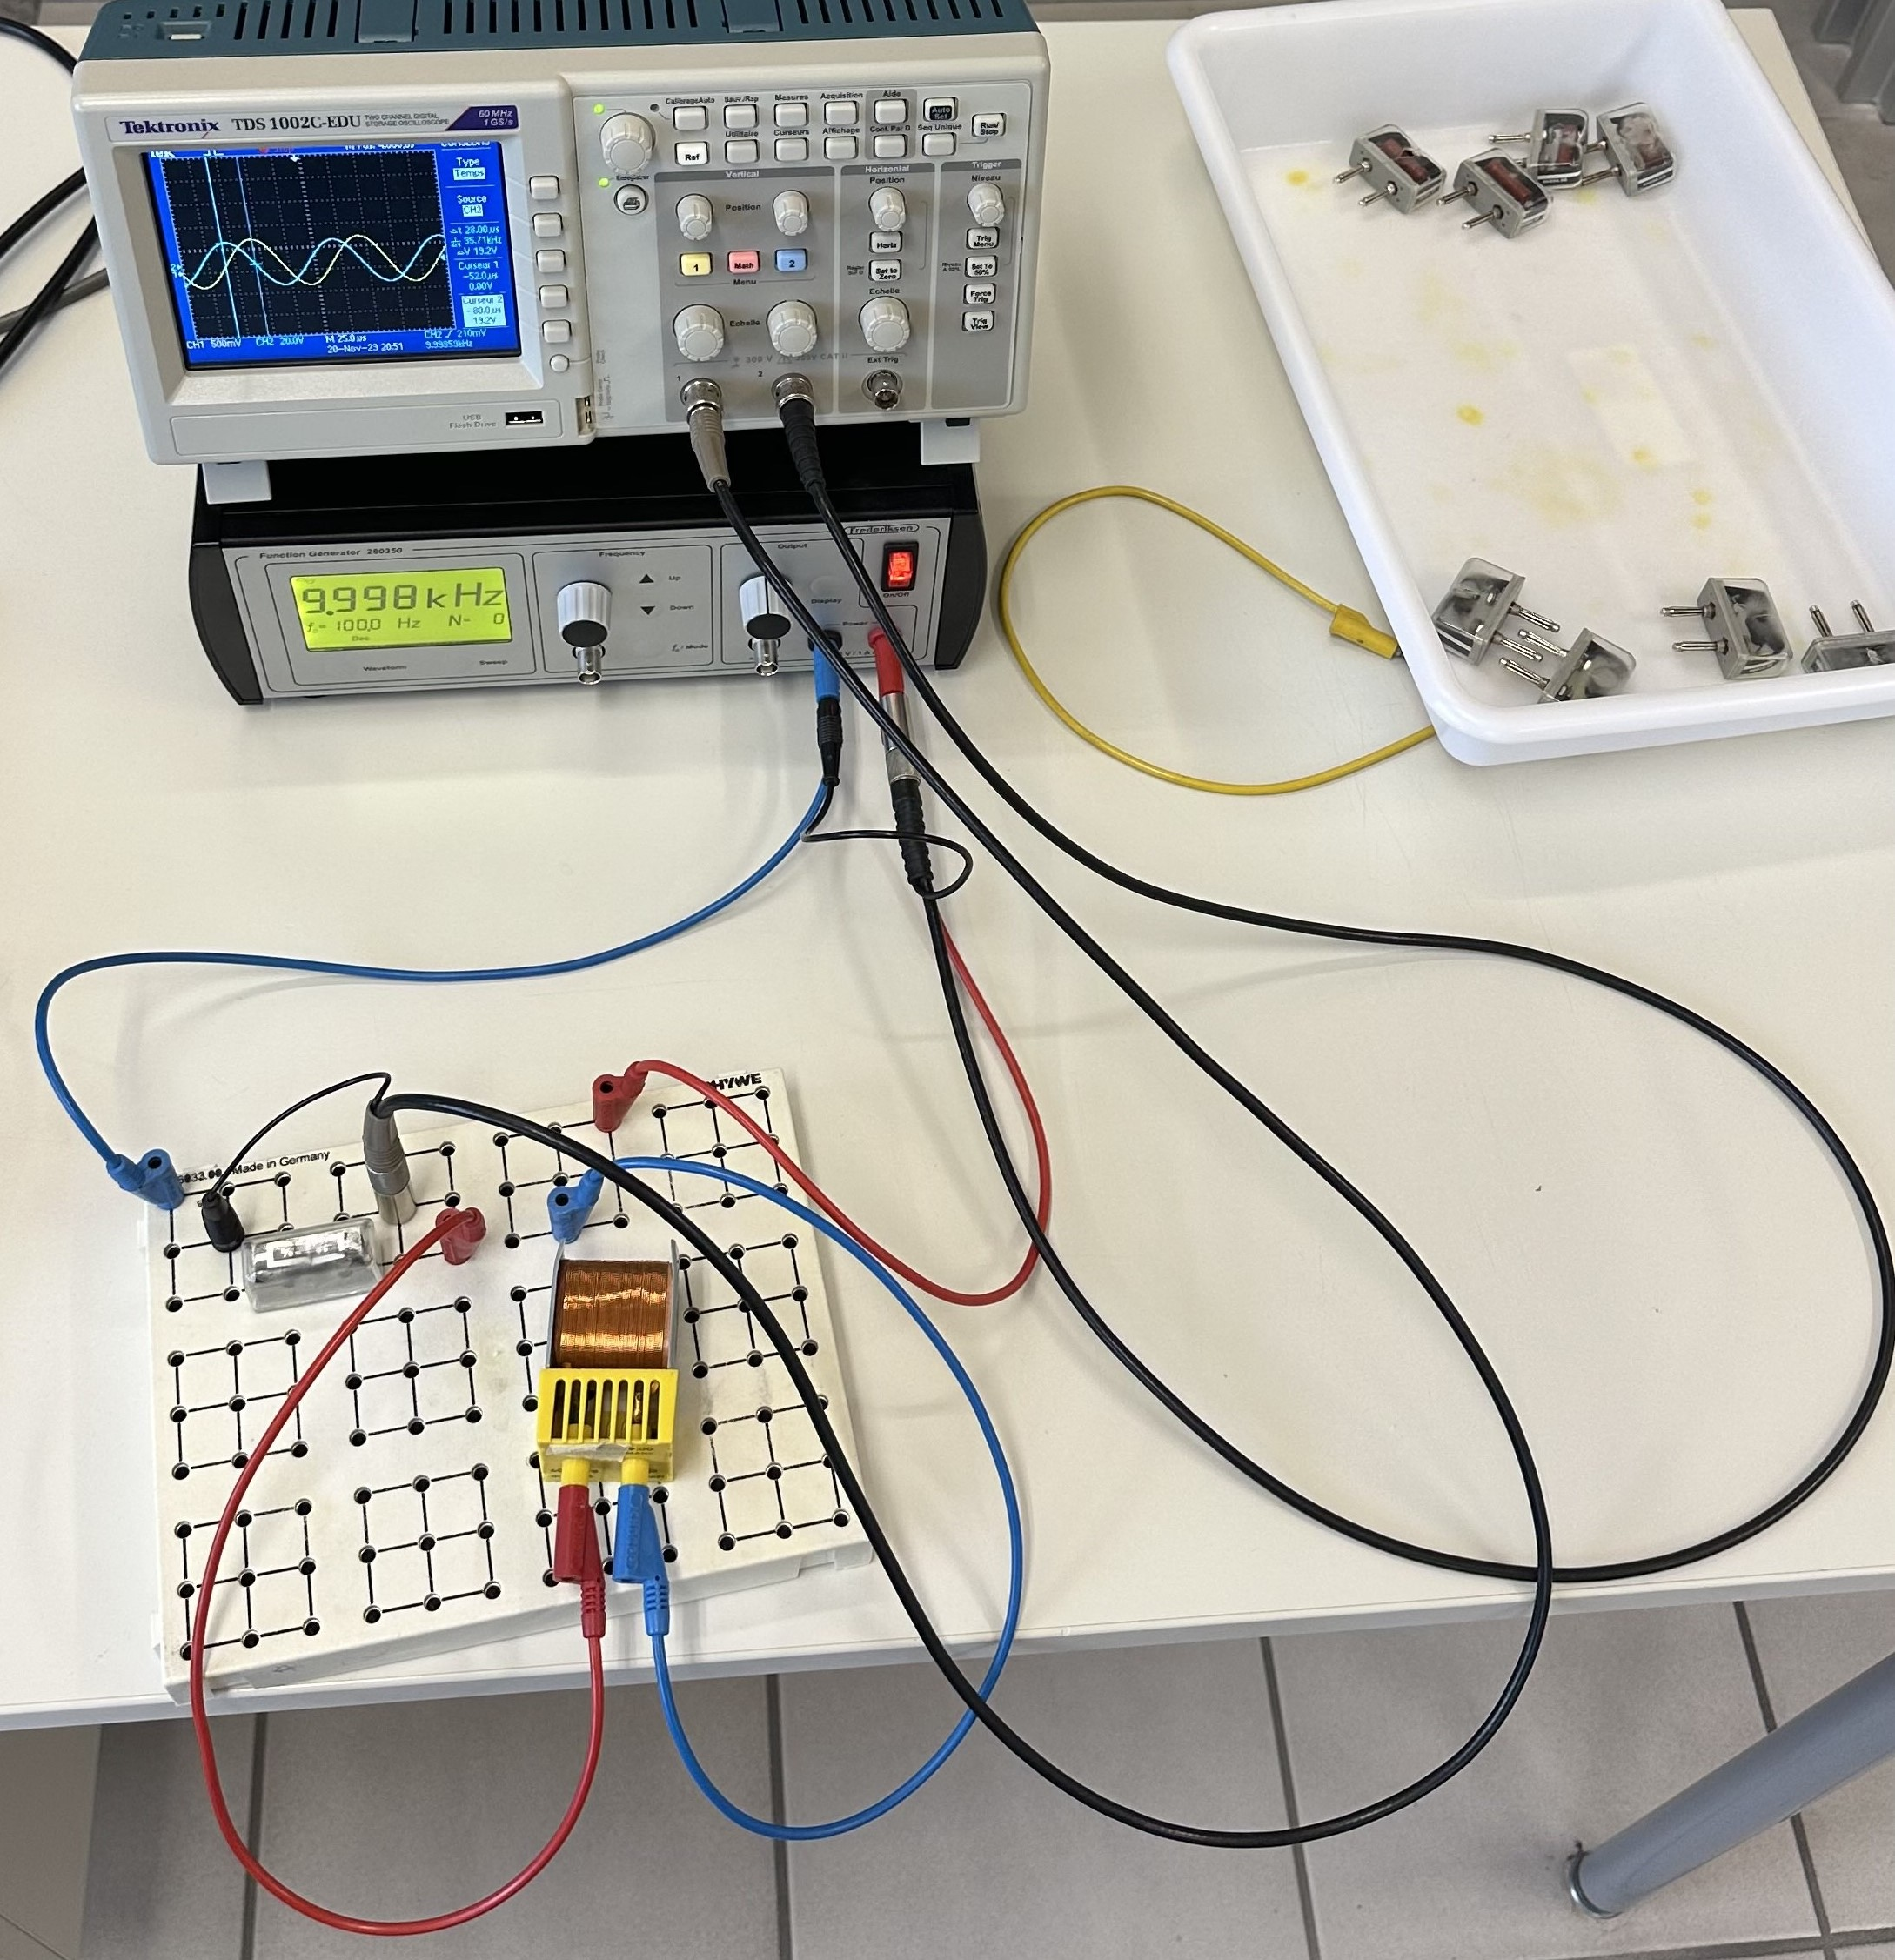
\includegraphics[width=0.6\textwidth]{phy_cir-RL.jpg}
    \caption{Photo du montage $RL$}
\end{figure}
\end{minipage}

\subsubsection*{Expérience 2 :}

\begin{minipage}{.5\textwidth}
\begin{figure}[H]
  \centering
    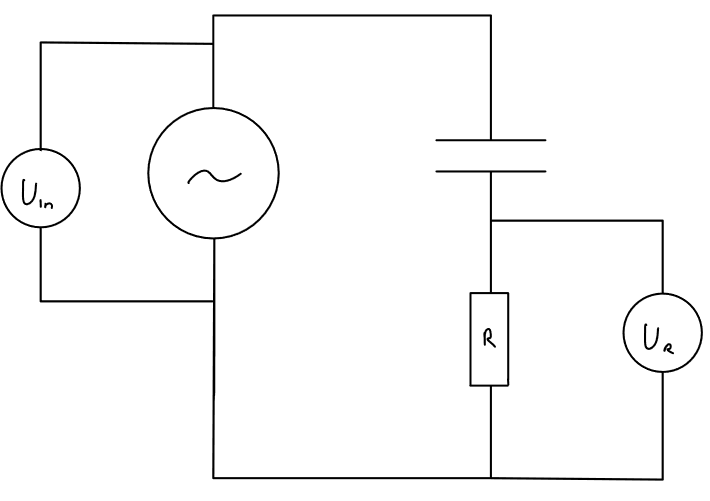
\includegraphics[width=0.8\textwidth]{phy_cir_RC.PNG}
    \caption{Schéma du circuit $RC$}
\end{figure}
\end{minipage}
\begin{minipage}{.5\textwidth}
\begin{figure}[H]
  \centering
    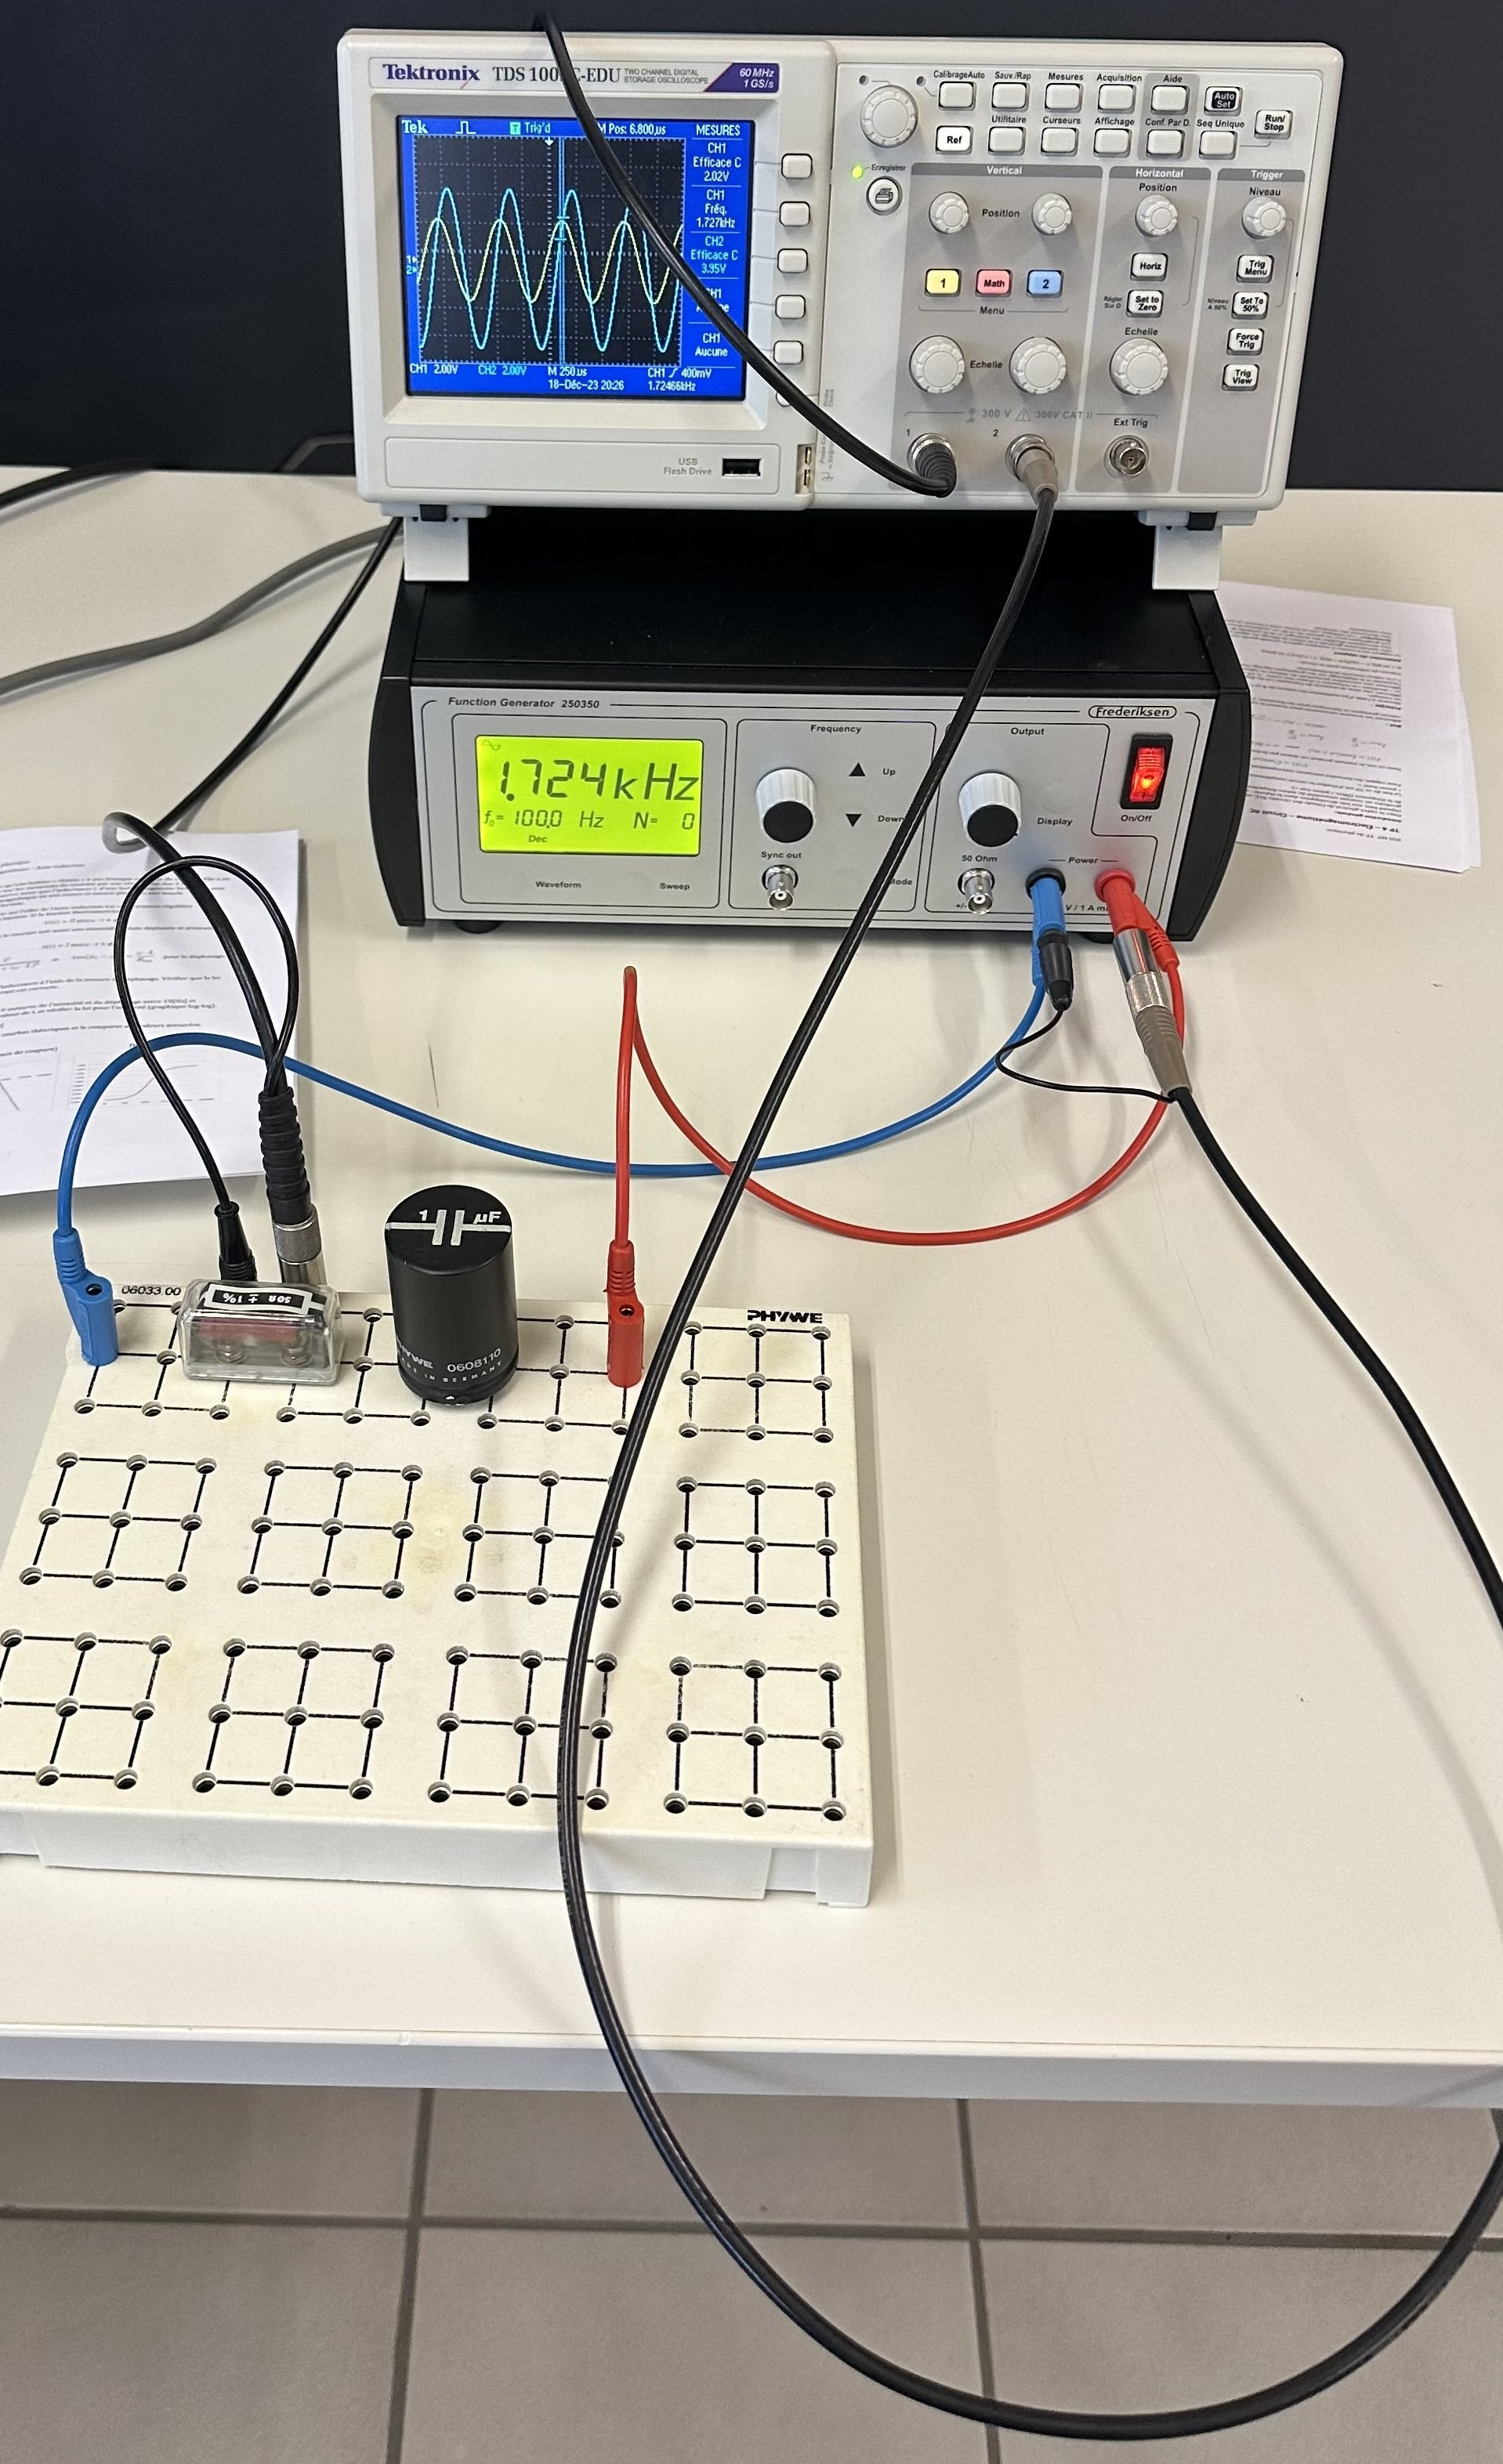
\includegraphics[width=0.6\textwidth]{phy_cir-RC.jpg}
    \caption{Photo du montage $RC$}
\end{figure}
\end{minipage}
